\documentclass{beamer}
% September 2014 
% Author: Dr Rachid Hourizi and Dr. Michael Wright 
% Department of Computer Science, University of Bath
\usepackage{listings}
\usetheme{Boadilla} 
\usepackage{fixltx2e}
\usepackage{hyperref}
\lstset{language=Java}

\begin{document}






\begin{frame}
\frametitle{Developping Interactive Classes: A digital clock}
\begin{center}
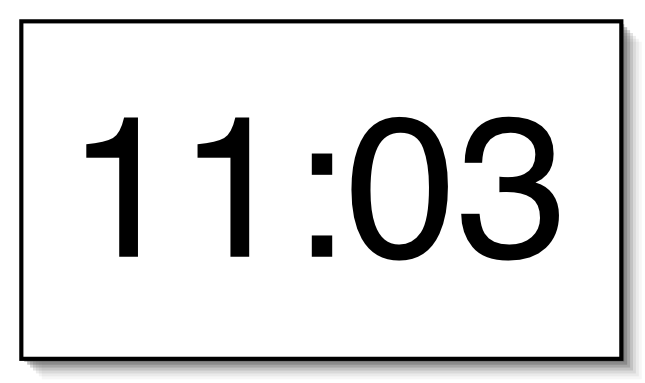
\includegraphics[height=5cm,keepaspectratio]{./figures/clock}
\end{center}
\end{frame}

\begin{frame}
\frametitle{Modularizing the clock display}
\begin{tabular}{lll}
\begin{minipage}{3cm}
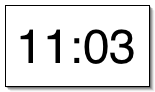
\includegraphics[height=1cm,keepaspectratio]{./figures/cl1} \end{minipage} & \mbox{}\hspace{1cm} & One four-digit display?\\
\mbox{}\\
\begin{minipage}{3cm}
Or two two-digit displays
\end{minipage}& & \begin{minipage}{3cm}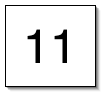
\includegraphics[height=1cm,keepaspectratio]{./figures/cl2}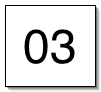
\includegraphics[height=1cm,keepaspectratio]{./figures/cl3}\end{minipage}
\end{tabular}
\end{frame}


\begin{frame}

\begin{itemize}
\item As we do so, we will consider challenges of abstraction and modularization:

\begin{itemize}
\item Abstraction is the ability to ignore details of parts to focus attention on a higher level of a problem.
\item Modularization is the process of dividing a whole into well-defined parts, which can be built and examined
separately, and which interact in well-defined ways.
\end{itemize}
\end{itemize}

\end{frame}

\begin{frame}

\begin{itemize}
\item A sensible approach if we go for 2*2-digit displays (`NumberDisplays') is to 

\begin{itemize}
\item write a NumberDisplays class which allows us to show any two digit number (i.e. a template for all NumberDisplays)

\item write a ClockDisplay class that creates two NumberDisplay instances
\item In other words, develop one class 
\item that (in turn) creates two instances of another class (two Objects)
\end{itemize}
\end{itemize}

\end{frame}

\begin{frame}
\frametitle{Object diagram}
\begin{center}
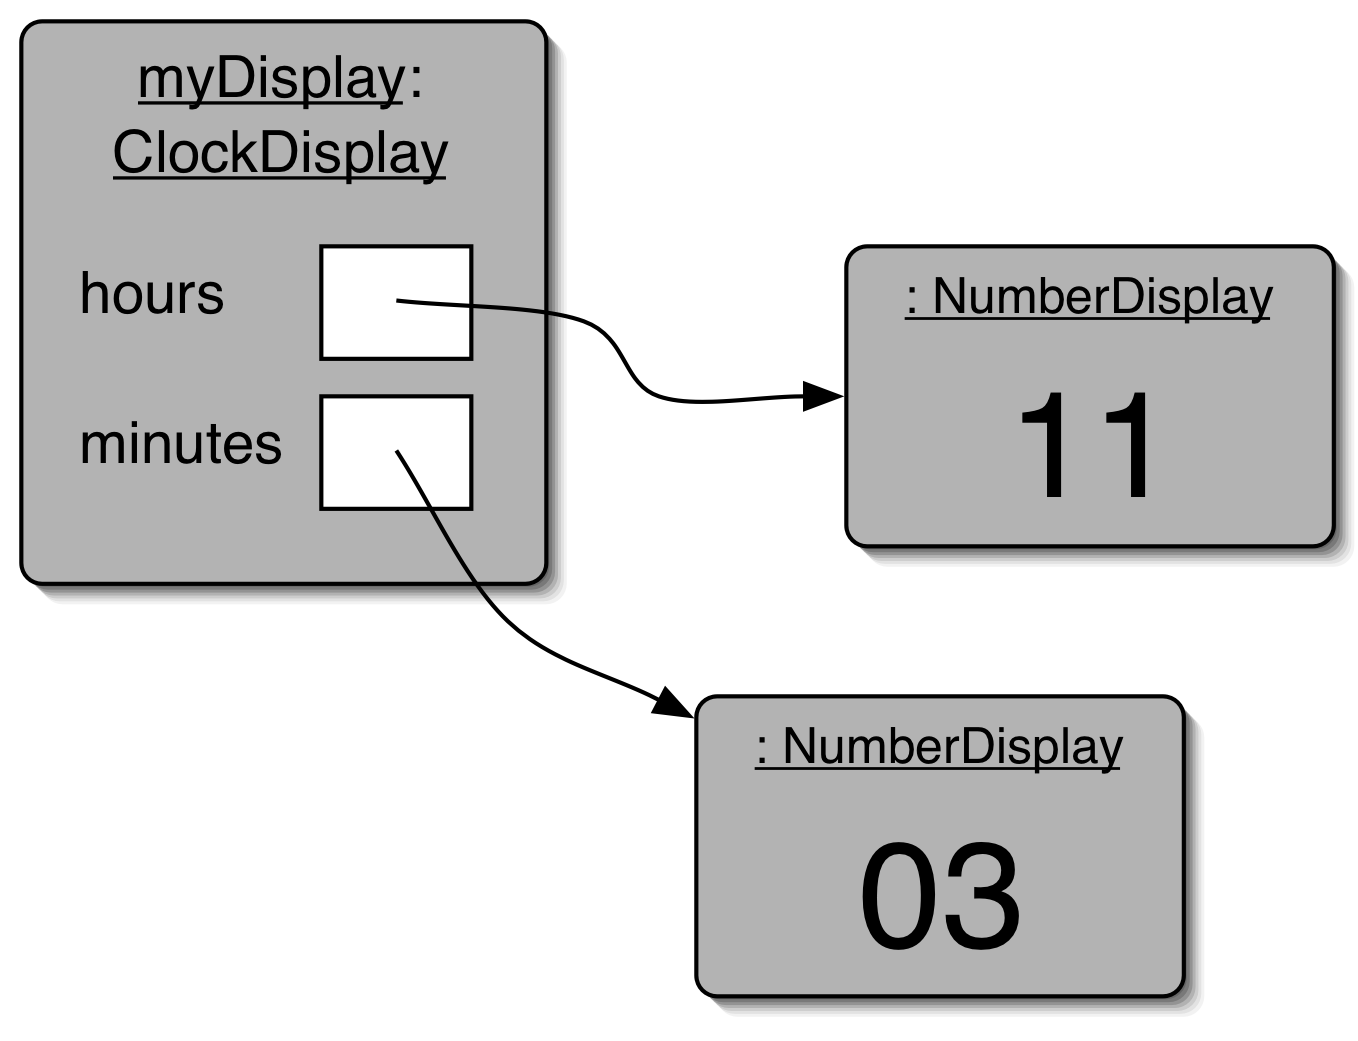
\includegraphics[height=5cm, keepaspectratio]{./figures/object}
\end{center}
\end{frame}

\begin{frame}
\frametitle{Class diagram}
\begin{center}
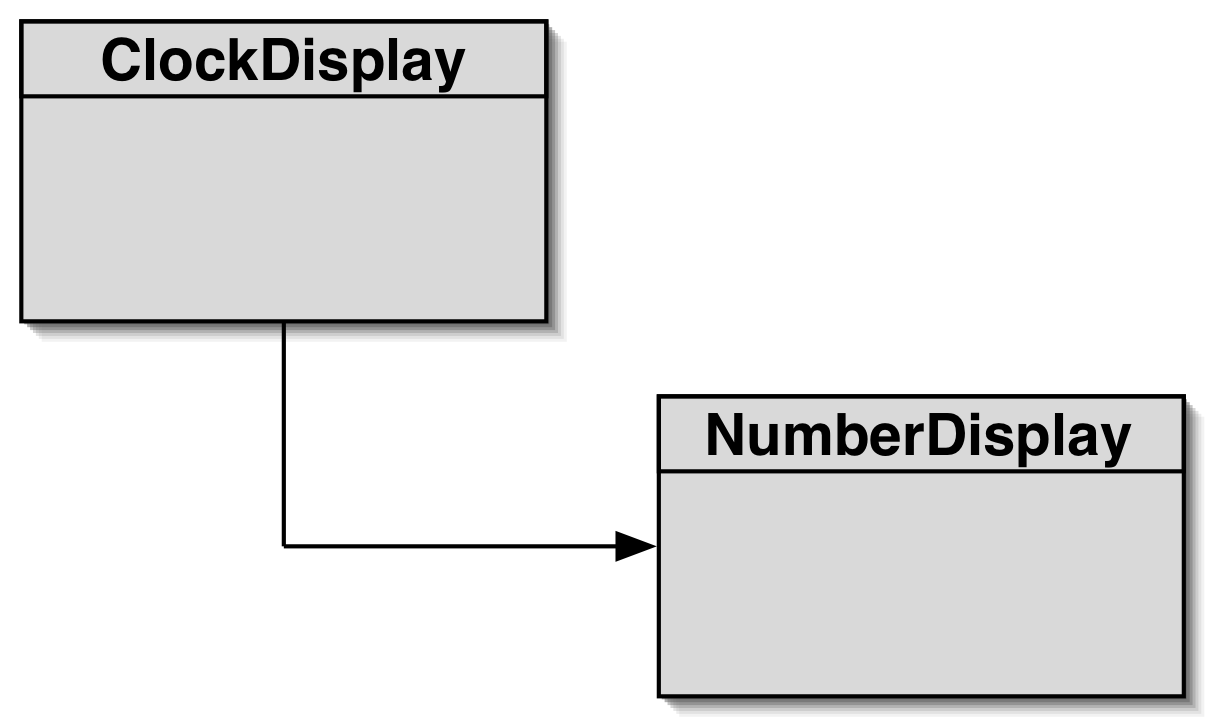
\includegraphics[height=5cm, keepaspectratio]{./figures/class}
\end{center}
\end{frame}


\begin{frame}[fragile]
\frametitle{Implementation: NumberDisplay}
\begin{lstlisting}[linewidth=6cm]
public class NumberDisplay
{
    private int limit;
    private int value;

    Constructor and
    methods omitted.
}
\end{lstlisting}
\end{frame}

\begin{frame}[fragile]
\frametitle{Implementation: ClockDisplay}
\begin{lstlisting}[linewidth=7cm]
public class ClockDisplay
{
    private NumberDisplay hours;
    private NumberDisplay minutes;

    Constructor and
    methods omitted.
}
\end{lstlisting}
\end{frame}


\begin{frame}

\begin{itemize}
\item Class Diagrams

\begin{itemize}
\item Show the classes of an application and the relationships
\item between them
\item Give information about the source code 
\item Static view of the program
\end{itemize}
\item Object Diagrams

\begin{itemize}
\item Show objects and their relationships at one moment in time during the execution of the program 
\item Dynamic view of the program
\end{itemize}
\end{itemize}

\end{frame}


\begin{frame}[fragile]

\begin{itemize}
\item We will use the incremental development approach described above:
\item Starting with class comments and a class definition for the NumberDisplay class (no import statements are needed)
\item all  of  the code needed to run a basic DigitalClock will be available on Moodle
\end{itemize}
\end{frame}

\begin{frame}[fragile]
\begin{itemize}
\item But first a few words on Java Strings:
\begin{itemize}
\item Java provides a String class
\item which in turn means that we can use String as a data type
\item Now that we know a little more about the construction of a Java class, we can guess that theString class provides us with at least one constructor
\item in fact it provides us with more than one
\item but the simplest is as follows:
\end{itemize}
\end{itemize}
\begin{block}{}
\small
\begin{lstlisting}
public class HelloWorld {

    public static void main(String[] args) {
    	
    	String greeting = "HelloWorld";
    	
        // Prints "Hello, World" to the terminal window.
        System.out.println(greeting);
    }

}

\end{lstlisting}
\end{block}
\end{frame}

\begin{frame}[fragile]
\begin{itemize}
\item The String class also provides us with accessors e.g. length
\end{itemize}
\begin{block}{}
\small
\begin{lstlisting}
public class HelloWorld {

    public static void main(String[] args) {
    	
    	String greeting = "HelloWorld";
	int strLength = greeting.length();
    	
        // Concatenates strLength to an emptyString and prints result to the screen
        System.out.println(""+strLength);
    }
}
\end{lstlisting}
\end{block}
\begin{itemize}
\item: Note the . notation used to call an accessor method of String greeting
\item: Note also the use of "+" to concatenate strLength to a String
\item: Finally, note the possibility of concatenating ints (or floats or chars) to a String - much easier than C.
\end{itemize}
\end{frame}

\begin{frame}[fragile]
\begin{itemize}
\item the use of + to concatenate Strings is extremely common in java
\item though a more formal concatente() method does exist
\item being able to concatenate any object to a string is also a big help when printing
\item this means that we do not need to use display formatting when printing combinations of Strings and values
\item we can simply print a long concatenation expression (starting with a String)
\end{itemize}
\begin{block}{}
\begin{lstlisting}
public class HelloWorld {

    public static void main(String[] args) {
    
        System.out.println(""+4.0+"Hello"+5);
    }
} 
\end{lstlisting}
\end{block}
\end{frame}

\begin{frame}
\begin{itemize}
\item What is actually happening is that the non String data is being converted to a String before printing
\item using the toString() method that is provided in each class
\item you may not like the way that Java converts data of other types to a String
\item but some conversion is always possible. 
\end{itemize}
\end{frame}

\begin{frame}
\begin{itemize}
\item Importantly, however, we cannot change the contents of a Java String once it has been created (Unlike a C String)
\item We cannot, for example, create a String and change the fourth letter.
\item The Java compiler will simply return an error if we try
\item We can describe this situation as one in which the Strings class does not provide us with mutator methods
\item Java Strings are, therefore described as \alert{immutable}
\item definition: An \alert{immutable data type} is a type whose state (contents) cannot be changed after creation.
\item defintion: A \alert{mutable} data type is a type whose data members, such as properties, data and fields, can be modified after its creation.
\end{itemize}
\end{frame}

\begin{frame}[fragile]
\begin{itemize}
\item Now we can return to developing a NumberDisplay class
\item following the iterative development approach, we will start with a very simple version of the code
\item i.e. a version which simply defines the class but provides neither fields nor methods
\end{itemize}
\tiny
\begin{block}{}
\begin{lstlisting}
/**
 * The NumberDisplay class represents a digital number display that can hold
 * values from zero to a given limit. The limit can be specified when creating
 * the display. The values range from zero (inclusive) to limit-1. If used,
 * for example, for the seconds on a digital clock, the limit would be 60, 
 * resulting in display values from 0 to 59. When incremented, the display 
 * automatically rolls over to zero when reaching the limit.
 * 
 * @author Michael Kolling and David J. Barnes
 * @version 2001.05.26
 */
public class NumberDisplay{
}
\end{lstlisting}
\end{block}

\end{frame}

\begin{frame}[fragile]

\begin{itemize}
\item followed by a definition of the fields needed by NumberDisplays
\end{itemize}

\begin{block}{}
\begin{lstlisting}
    private int limit;
    private int value;
\end{lstlisting}
\end{block}

\end{frame}

\begin{frame}[fragile]

\begin{itemize}
\item Next, we define constructors for the NumberDisplays
\end{itemize}

\begin{block}{}
\begin{lstlisting}
    /**
     * Constructor for objects of class NumberDisplay
     */
    public NumberDisplay(int rollOverLimit)
    {
        limit = rollOverLimit;
        value = 0;
    }
\end{lstlisting}
\end{block}

\end{frame}
\begin{frame}[fragile]

\begin{itemize}
\item Next, we can define the Accessors for the Number Display class
\end{itemize}

\scriptsize
\begin{block}{}
\begin{lstlisting}
    /**
     * Return the current value.
     */
    public int getValue()
    {
        return value;
    }

    /**
     * Return the display value (that is, the current value 
     * as a two-digit String. If the value is less than ten, 
     * it will be padded with a leading zero).
     */
    public String getDisplayValue()
    {
        if(value < 10)
            return "0" + value;
        else
            return "" + value;
    }
\end{lstlisting}
\end{block}

\end{frame}

\begin{frame}[fragile]

\begin{itemize}
\item ...and finally the mutators
\end{itemize}

\scriptsize
\begin{block}{}
\begin{lstlisting}
   /**
     * Set the value of the display to the new specified value. 
     * If the new
     * value is less than zero or over the limit, do nothing.
     */
    public void setValue(int replacementValue)
    {
        if((replacementValue >= 0) && (replacementValue < limit))
            value = replacementValue;
    }

    /**
     * Increment the display value by one, rolling over 
     * to zero if the limit is reached.
     */
    public void increment()
    {
        value = (value + 1) % limit;
    }

\end{lstlisting}
\end{block}

\end{frame}

\begin{frame}

\begin{itemize}
\item Having written code that defines the NumberDisplay class
\item i.e. a template for all NumberDisplay Objects
\item we can now write a ClockDisplay class 
\item That uses two NumberDisplay Objects
\end{itemize}

\end{frame}

\begin{frame}[fragile]

\tiny
\begin{block}{}
\begin{lstlisting}
/**
 * The ClockDisplay class implements a digital clock display for a
 * European-style 24 hour clock. The clock shows hours and minutes. The 
 * range of the clock is 00:00 (midnight) to 23:59 (one minute before 
 * midnight).
 * 
 * The clock display receives "ticks" (via the timeTick method) every minute
 * and reacts by incrementing the display. This is done in the usual clock
 * fashion: the hour increments when the minutes roll over to zero.
 * 
 * @author Michael Kolling and David J. Barnes
 * @version 2001.05.26
 */
public class ClockDisplay
{
}
\end{lstlisting}
\end{block}

\end{frame}

\begin{frame}[fragile]

\begin{block}{}
\begin{lstlisting}
    private NumberDisplay hours;
    private NumberDisplay minutes;
    private String displayString;    
\end{lstlisting}
\end{block}

\end{frame}

\begin{frame}[fragile]
\tiny
\begin{block}{}
\begin{lstlisting}
 /**
     * Constructor for ClockDisplay objects. This constructor 
     * creates a new clock set at 00:00.
     */
    public ClockDisplay()
    {
        hours = new NumberDisplay(24);
        minutes = new NumberDisplay(60);
        updateDisplay();
    }

    /**
     * Constructor for ClockDisplay objects. This constructor
     * creates a new clock set at the time specified by the 
     * parameters.
     */
    public ClockDisplay(int hour, int minute)
    {
        hours = new NumberDisplay(24);
        minutes = new NumberDisplay(60);
        setTime(hour, minute);
    }
\end{lstlisting}
\end{block}

\end{frame}

\begin{frame}[fragile]
\tiny
\begin{block}{}
\begin{lstlisting}
     /**
     * This method should get called once every minute - it makes
     * the clock display go one minute forward.
     */
    public void timeTick()
    {
        //some code
    }

    /**
     * Set the time of the display to the specified hour and
     * minute.
     */
    public void setTime(int hour, int minute)
    {
        //some code
    }
\end{lstlisting}
\end{block}

\end{frame}

\begin{frame}[fragile]
\tiny
\begin{block}{}
\begin{lstlisting}
     /**
     * Return the current time of this display in the format HH:MM.
     */
    public String getTime()
    {
        //some code
    }
    
    /**
     * Update the internal string that represents the display.
     */
    private void updateDisplay()
    {
        //some code
    }
\end{lstlisting}
\end{block}

\end{frame}

\begin{frame}

\begin{itemize}
\item Note: The ClockDisplay class creates and uses two NumberDisplay Objects

\begin{itemize}
\item new NumberDisplay(parameter-list)

\begin{itemize}
\item creates a new NumberDisplay Object
\item i.e. we execute the constructor of that class
\item this involves creating sufficient memory to store the values of primitive instance variables and references to
object instance variables.
\end{itemize}
\end{itemize}
\end{itemize}

\end{frame}


\begin{frame}

\begin{itemize}
\item Public methods:

\begin{itemize}
\item public void increment() can be called externally
\end{itemize}
\item Private methods

\begin{itemize}
\item private void updateDisplay()
\item can only be called internally used for auxiliary methods
\end{itemize}
\end{itemize}

\end{frame}

\begin{frame}[fragile]

\begin{block}{}
\begin{lstlisting}
public class Point {
    public int x = 0;
    public int y = 0;
        
    //constructor
    public Point(int x, int y) {
        this.x = x;
        this.y = y;
    }
}
\end{lstlisting}
\end{block}

\end{frame}

\begin{frame}

\begin{itemize}
\item Implementing a test program:

\begin{itemize}
\item The purpose of a test program is to verify that one or more methods have been implemented correctly
\item A test program calls methods and checks that they return the expected results.
\end{itemize}
\end{itemize}

\end{frame}\begin{frame}

\begin{itemize}
\item A test program contains the following steps:

\begin{itemize}
\item Provide a tester class
\item Supply a main method
\item Inside the main method, create one or more objects
\item Apply methods to the objects
\item Display the results of the method calls - if needed
\item Display the value that you expect to get - if possible
\end{itemize}
\end{itemize}
\end{frame}


\begin{frame}[fragile]
\scriptsize
\begin{block}{}
\begin{lstlisting}
/**
 * This cTest class instantiates a Java digital clock from Kolling  
*  & Barnes ClockDisplay and NumberDisplay Classes. 
* It prints the time generated by those classes to the screen 
*  approximately every second.
*/
public class cTest{

static boolean isActive=true;

//main method
public static void main(String args[]){

    ClockDisplay myClock = new ClockDisplay();	
        do{
            myClock.timeTick();
            System.out.println(myClock.getTime());
            wait(60);			
        }
        while(isActive);	
}
\end{lstlisting}
\end{block}
\begin{itemize}
\item Note the use of do while (covered in more depth later in the course but similar to C)
\end{itemize}



\end{frame}

\begin{frame}[fragile]
\begin{itemize}
\item note the use of System.currentTime.Millis() which returns the current system time in milliseconds
\end{itemize}
\scriptsize
\begin{block}{}
\begin{lstlisting}
//crude pausing method from http://blog.qarea.com/development/java-development/how-to-make-java-wait/
public static void wait (int k){
	
        long time0=0; 
        long time1=0;

        time0 = System.currentTimeMillis();

        do{
            time1 = System.currentTimeMillis();
        }
       while ((time1-time0) < k * 1000);
    }
}
\end{lstlisting}
\end{block}

\end{frame}

\begin{frame}
\begin{itemize}
\item Exercise:
\begin{itemize}
\item How would you adjust the DigitalClock code to hold, update and display the time in hours, minutes and seconds (HH:MM:SS) rather than just hours and minutes?
\item add comments to the code provided that describe each of the changes that you would have to make
\item where you are able, also provide the Java code to make these changes
\end{itemize}
\end{itemize}
\end{frame}




\end{document}
